\documentclass{acm_proc_article-sp}
\usepackage[hyphens]{url}
\usepackage{hyperref}
\usepackage{dblfloatfix}
\begin{document}

\title{Applying Desktop Race Detector Techniques to Mobile Systems}
\numberofauthors{2}
\author{
\alignauthor Dan Jonik\\
\affaddr{University of Michigan, Ann Arbor}\\
\email{djonik@umich.edu}
\and
\alignauthor Jason Varbedian\\
\affaddr{University of Michigan, Ann Arbor}\\
\email{jpvarbed@umich.edu}
}
\date{25 April 2012}
\maketitle

\begin{abstract}
Mobile systems have recently become prevalent with more smart phones being sold than any other computing device. Development for these systems has increased as fast as the sales with applications and systems requiring more powerful hardware. Smart phones are being released with multicore architectures and come with the same multithreaded programming difficulty as desktop systems face. Debugging and developing applications for these multicore mobile platforms is a difficult task and few if any tools exist specifically for concurrency detection.
 
This paper presents an implementation and port of the FastTrack race detector for the Android mobile system. Android lacks any true instrumentation library and most Java instrumentation is done at runtime instead of compile which don't work on Android. The tool is able to detect errors in simple applications we wrote ourselves while running on an Android emulator. 
\end{abstract}

\section{Introduction}
Multiple cores and multithreaded programming has become the standard on desktop systems. Chips have had to increase the number of cores to increase computing power. To take advantage of these cores multiprogramming is often used. Programming for multiple cores is often non-trivial even for so-called 'embarrassingly parallel' calculations. The challenge is greater for large applications and services like browsers and servers. Several tools have been developed for desktop systems to help with debugging these programs.
 
Smart phones are becoming multicore and apps are running  with multiple threads. Many data race detectors and multithreaded programming tools have been developed for desktop systems, but few exist for mobile systems. The introduction of multicore processors to mobile space introduces non-deterministic bugs. These bugs inhibit development as the current technique for solving non-deterministic concurrency errors is the use of exhaustive, expensive, and time-consuming tests. These tools will run an app for a significant period of time with many different environment variables and output diagnostic logs. There are exponentially-many interleavings to explore and it can be difficult to pinpoint when and where an error occurred; additionally, it is just as difficult to reproduce a bug once it has been found. There is an obvious need for tools to air developers in finding data races before they manifest into multithreaded bugs.

There have been many race detectors, record and replay systems, and other tools to monitor and debug concurrent programs for desktop systems. In our research and our time working in industry with commercial Android products, we have found no such tools for mobile systems. It is possible there are proprietary tools that Apple and Microsoft use for their mobile systems, bu there isn't yet a publicly-available one for Android.
 
Our hypothesis is that data race techniques implemented on desktop systems can be applied to mobile systems. Our project ports a low-overhead, fast, and thorough dynamic race detector called FastTrack that runs on the Java Virtual Machine to Android's Dalvik Virtual Machine. The detector FastTrack \cite{Flanagan2009} implements an algorithm that, used with the dynamic analysis framework RoadRunner, can monitor memory accesses and synchronization operations in concurrent Java programs. FastTrack checks that programs follow a \emph{happens-before} relationship[citation] with lightweight vector clocks that, in most cases, use constant space and time operations. RoadRunner provides an API for communicating an event stream to back-end analysis tools; FastTrack monitors this event stream to monitor an application's behavior. The tool makes debugging multithreaded applications much faster and easier to fix by providing detailed information about each detected data race.
 
In this paper we make two contributions:
\begin{enumerate}
\item Describe issues with porting data race detection systems to Android
\item A partial port of FastTrack and RoadRunner to Android
\end{enumerate}

The rest of the paper is organized as follows. The following section reviews tools used for multithreaded program debugging and development and explains our choice of which tool is the most appropriate to port to Android. Section 3 describes the  RoadRunner instrumentation framework. Section 4 explains the algorithm used by FastTrack to build and monitor a \emph{happens-before} relation. Section 5 presents the modifications we made to the FastTrack tool to run it on Android, followed by an evaluation of our work in Section 6. Section 7 discusses possible areas of future work and extensions that could be added to our work.

\section{Survey of Existing Tools}
There are many techniques for detecting data races and providing record and replay capabilities for desktop multithreaded applications. We surveyed different tools and systems to determine which would be the most appropriate for use in a mobile computing environment. Mobile systems, compared to desktops and laptops, have less memory and fewer cores since energy is a limiting resource for system performance; therefore, we were most interested in debugging tools that had relatively small memory footprints and performance overheads. False positives, when a benign data race is erroneously reported as an error, greatly limit a tool's usefulness and usability, so we favored tools that guaranteed to report only legitimate errors. Several debugging tools require developers to make modifications to their application's source code before the tool can be used. This is not only a burden to the programmer, but also could possibly introduce additional bugs that were not previously present. Our ideal tool requires no source code modifications to preserve both correctness and usability. Our analysis of five different desktop multithreaded debugging tools is presented below.

\begin{description}
\item[DoublePlay] \cite{Veeraraghavan2012} is a deterministic system that provides guaranteed record and replay with minimal overhead at the cost of using more cores.  It does so by running the original multithreaded program on half the of cores and taking "checkpoints", while at the same time running multiple time-slices of a single-processor execution on the other half of the cores. The key insight is that by running different time-slices of a program each on their own individual core, multithreaded code can be executed and then replayed deterministically without a severe performance hit. In case of a mismatch between the single-processor execution and the multiprocessor execution, both executions are rolled back to the last checkpoint and restarted. DoublePlay is very effective because it offers full replay capabilities to multithreaded software, does not report false positives, and introduces little slow down. However, since DoublePlay is based on the assumption that the system on which it is running has unused cores (an assumption that most definitely does not apply to mobile systems), we decided that it was not the best option for porting to Android. 

\item[Eraser] \cite{Savage1997} is a system used to detect data races in programs that use locks for synchronization by using the \emph{lock-set} algorithm. Eraser keeps track of which locks are held at each access to a shared object; if there is ever an access in which the set of locks held is empty, a data race is reported. Unfortunately, there are several circumstance in which false positives may be reported, such as user-implemented synchronization techniques. When these situations arise, developers are forced to add statements to their code telling Eraser to ignore certain objects and accesses. Eraser implements a straightforward data race detection algorithm, but ultimately fails on two of our predefined criteria, requiring source code modification and reporting of false positives.


\item[Kendo]  \cite{Olszewski2009} is a tool that guarantees weak determinism for multithreaded applications. It modifies the POSIX thread library to ensure a deterministic order of all lock acquisitions for a given set of inputs based on the current progress of each thread. Unfortunately, Kendo requires programmers to insert library calls around intentionally racy reads to flag them as benign so that Kendo ignores them. Perhaps an even bigger limitation is that Android applications run on the native Java Thread library; therefore, porting Kendo to Android would require a complete reimplementation as well as redefining a native Java library, which is discourage and limits the system's portability.


\item[CHESS] \cite{Musuvathi2008} is a system for systematically testing concurrent systems for bugs that appear only in certain thread interleavings. It does so by taking control of the thread scheduler and exhaustively enumerating all possible thread interleavings. To reduce the number of program execution paths that must be explored, threads are preempted only at certain key instructions (instead of at every instruction) that are most likely to be central to any bugs that appear. CHESS offers no false positives and near-complete code coverage, but requires the creation of wrappers to allow the tool to run on top of different development platforms  Additionally, it is a resource-hungry  application which would experience performance problems on mobile devices.


\item[FastTrack] \cite{Flanagan2009} is able to monitor any concurrent Java program and report only true data races with full \emph{happens-before} coverage. By instrumenting compiled Java class files at load time, it uses a shadow memory system to watch all synchronization and memory  operations. It is able to identify the type of data race that has occured, which threads were involved, and which variable was the cause.  FastTrack uses a shortened version of vector clocks, known as \emph{epochs}, to monitor the \emph{happens-before} relationship. \emph{Epochs} reduce the memory overhead of the system, as well as speed up the comparison operations used to check for data races. FastTrack is the ideal algorithm choice for an Android race detector since it requires no source modifications, it has a small memory and performance overhead, and it reports only true data races.
\end{description}

\section{RoadRunner}
RoadRunner is a dynamic analysis framework for monitoring concurrent Java programs. It provides an interface for compiled Java bytecode instrumentation without requiring any changes to the underlying virtual machine. RoadRunner outputs updated class files that have additional function calls to the RoadRunner framework wrapped around each synchronization operation and memory access. When an instrumented class file is executed, it will be making calls to RoadRunner, which then broadcasts the events to any programs, such as FastTrack, that have subscribed to the event stream. These programs can then monitor and handle the events in whatever way they desire.


\subsection{RoadRunner API}
RoadRunner provides an abstract class, Tool, that allows different types of programs to be built on top of RoadRunner. Inside of this class, developers must specify how to handle different types of events that come from RoadRunner by overwriting virtual event handler functions; although a wide variety of events are broadcast, tools only need to write handlers for the events that they care about. FastTrack is an extension of the Tool class that monitors all memory operations and synchronization operations. The fastTrack event handlers use the events to construct a \emph{happens-before} graph which is then used to monitor for data races.


\subsection{Instrumentation}
RoadRunner uses the ASM \cite{Bruneton02} library to instrument Java classes at load time from a compiled Java .class file. A shadow variable is created for each static member of the class, as well as getter and putter functions to access the variable. \emph{ShadowThread} objects and function calls are inserted to the class to keep track of variable accesses between threads. An example instrumented class is below in Figure \ref{instrumentation}.
  \begin{figure}[h]
    \centering
    \begin{minipage} [h] {7.5cm}
      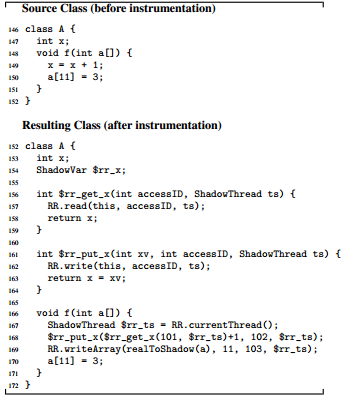
\includegraphics[scale=.9]{instrumentatin}
      \caption{An example of an instrumented class. A ShadowVar \emph{x} is created along with its get and put functions. The current thread is stored in the ShadowThread and used in the access operations.\label{instrumentation}}
    \end{minipage}
  \end{figure}


\section{FastTrack}
FastTrack is an extension of RoadRunner that uses a modified \emph{happens-before} relationship to monitor concurrent programs. It monitors an event stream and reports if there are any race conditions. A \emph{happens-before} relation is represented by vector clocks \cite{citeulike} which use considerable memory and require costly comparison operations. Given an application with  \emph{n} threads, each vector clock requires \emph{O(n)} storage space and each vector clock comparison operation requires \emph{O(n)} time. Previous tools have chosen between the precision (no false positives) and large overhead of full vector clocks and the imprecision which produces many false alarms. It can be difficult to identify real errors in a large least of fake ones. Fasttrack provides a precise race detector with low overhead by using lightweight vector clocks that in most cases use constant time and space operations.

\subsection{Happens-Before Relationship}
The Happens-Before relationship is an important relation in distributed and parallel systems. Formulated by Leslie Lamport \cite{Lamport1978}, is a "relation between the result of two events, such that if one event should happen before another event, the result must reflect that even if those events are in reality executed out of order." If the happens-before relation is respected during execution, then a program has no data races.

\subsection{Fasttrack Algorithm}
The key to the Fasttrack algorithm's low overhead is the observation that most operations don't need a full vector clock, just the information about the last access. The algorithm stores an epoch for the last access in most cases which is a tuple of the vector clock time (c)  and thread (t) denoted c@t. The idea is that writes are ordered until there is a race so the algorithm just needs to check if a new read or write proceeds the last recorded epoch. Let V1 and V2 be the vector clocks of thread 1 and 2, respectively.
 \begin{figure}[h]
    \centering
    \begin{minipage} [b] {8cm}
      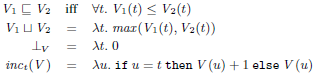
\includegraphics[scale=1]{termin}
    \end{minipage}
    \begin{minipage} [b] {7cm}
      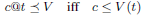
\includegraphics[scale=1]{lessthan}
	\caption{Terminology\label{termin}}
    \end{minipage}
  \end{figure}
Figure \ref{trace} shows a sample trace and how the epochs Wx and Rx are updated between two threads with vector clocks C0 and C1.
 \begin{figure}[h]
    \centering
    \begin{minipage} [b] {7.5cm}
      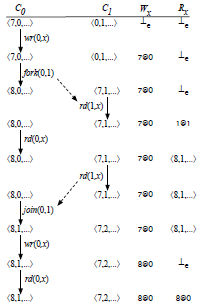
\includegraphics[scale=1]{full_trace}
      \caption{Instrumented Class\label{trace}}
    \end{minipage}
  \end{figure} 
Figures \ref{read} and \ref{write} shows how Fasttrack handles reads and writes for different types of accesses and the observed percentage from benchmarks. Since read operations aren't always ordered (one could finish after with a earlier clock time) and a program would still be correct, it is sometimes necessary to keep a full vector clock to make sure the very last read isn't changed by a write. Less than 0.1\% of writes and reads require a full vector clock which is when multiple reads happen followed by a write.
 \begin{figure}[h]
    \centering
    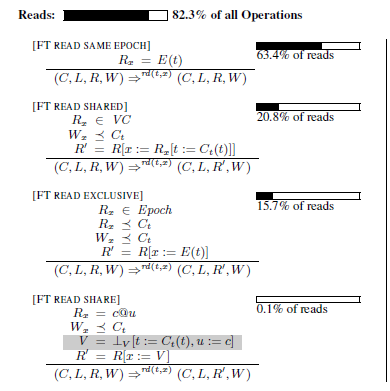
\includegraphics[scale=.5]{fast_read}
	\caption{Read Accesses\label{read}}
 \end{figure}
\begin{figure}[h]
    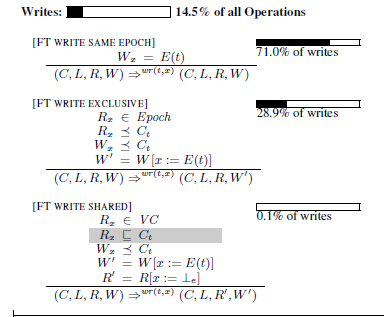
\includegraphics[scale=.5]{fast_write}
\caption{Write Accesses\label{write}}
  \end{figure}

\section{Implementation}
This section describes the changes we made to Fasttrack and RoadRunner to work with Android applications on Android 2.1. We chose Android 2.1 because its emulator and release are stable and has many tools available. The most significant hurdle with porting these systems is that Java.lang.instrumentation is not included in Android. We had to get around this by doing instrumentation and transformation at compile time and force metadata to be created.

An app must run on the host machine to have its classes instrumented permanently so we have to unpackage Android files back to Java class files. The class files are run on a host Linux machine and the class files are instrumented. The Android app is then rebuilt with Fasttrack and RoadRunner libraries and run on the target device or emulator.   

\section{Evaluation}
In evaluating our project, we looked at increase in code size, runtime overhead, ease of use, and bugs found. We were able to instrument class files and prepare simple class files for running on Android.

\section{Conclusion}
We believe that the Fasttrack algorithm is a good fit for mobile systems, but the instrumentation system of RoadRunner and the lack of instrumentation in Android limits its effectiveness. If the RoadRunner system was rewritten to always statically load classes or an instrumentation system was made for Android, then more apps could be monitored.

\bibliographystyle{acm}
\bibliography{monitor}
\end{document}